%================================================================
\section{Theory}\label{sec:Theory}
%================================================================

%----------------------------------------------------------------
\subsection{Project Theory 1}\label{sec:project theory}
%----------------------------------------------------------------

\subsection{Boltzmann machines}
A \textit{Boltzmann machine} (BM) is an undirected probabilistic graphical model with stochastic continuous or discrete nodes. It consists of one visible and one hidden layer, which are both inter- and intraconnected, meaning that there are weight matrices that represents the strength of the interactions between the nodes (both within the same layer and connections to the nodes in the other layer). The Boltzmann machine is a generative model as it allows generating new samples from a learned distribution. These properties are useful in our search for a ground state wave function, however, the Boltzmann machine is hard to train. We will therefore employ a \textit{restricted Boltzmann machine} to do our bidding.  \autoref{fig:vis_BM} is a simple representation of a BM network, where all the nodes are connected. 

\begin{figure}[H]
\begin{center}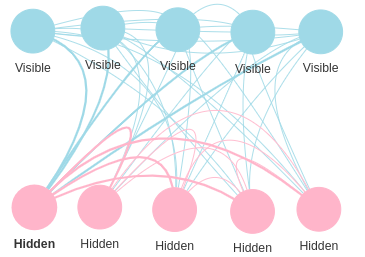
\includegraphics[scale=0.5]{latex/latex-report/Images/vis_BM.png}
\end{center}
\caption{Simple visualization of a BM network with a visible layer and hidden layer, both containing five nodes. The links between the nodes are weighted, and they are all contained within a weight matrix, $W$. Every link is undirected, as the connections go both ways.}
\label{fig:vis_BM}
\end{figure}

\subsection{Restricted Boltzmann Machines}



\begin{figure}[H]
\begin{center}\includegraphics[scale=0.5]{latex/latex-report/Images/rbm_.png}
\end{center}
\caption{Simple visualization of a BM network with a visible layer and hidden layer, both containing five nodes. The links between the nodes are weighted, and they are all contained within a weight matrix, $W$. Every link is undirected, as the connections go both ways.}
\label{fig:vis_BM}
\end{figure}




